\chapter{RESULTADOS}
\label{Resultados}

Neste trabalho, são consideradas as tecnologias \textit{open-source} utilizadas para prover conteúdo na Internet, assim como, as boas práticas de desenvolvimento para aplicações \textit{Web} modernas apresentadas ao longo deste trabalho. São descritos neste capítulo, os resultados dos experimentos propostos no Capítulo~\ref{Proposta}, que são: Estratégias para a redução do \textit{payload}; Aplicação da técnica de \textit{Critical} CSS.

Os resultados esperados para os experimentos têm como objetivo reduzir o consumo de tempo na renderização de páginas e na resposta das requisições HTTP. Portanto, são utilizados os conceitos explanados e aplicados às boas práticas introduzidas ao longo desde trabalho.

A primeira aplicação prática, proposta na Subseção~\ref{SubCriticalCSS}, descreve a importância de haver separação do CSS crítico. Em outras palavras, há um conjunto de regras de formatação de página que são indispensáveis para a renderização inicial do documento HTML junto ao DOM. Em seguida, após a renderização do conteúdo crítico, os demais componentes visuais e folhas de estilo são requisitadas através de AJAX. Assim, o motor de renderização do navegador executa com mais fluidez a exibição da página devido à otimização no tamanho da árvore DOM a ser renderizada. Esta otimização é impulsionada pela aplicação da técnica de \textit{Critical} CSS. Entretanto, os resultados não contêm dados de requisições realizadas após a renderização inicial. Na Figura~\ref{fig:withoutcritical}, pode-se observar o gráfico de desempenho de renderização antes da técnica ser implementada.

\begin{figure}[th]
\centering{
\caption{Desempenho antes do \textit{Critical} CSS.}
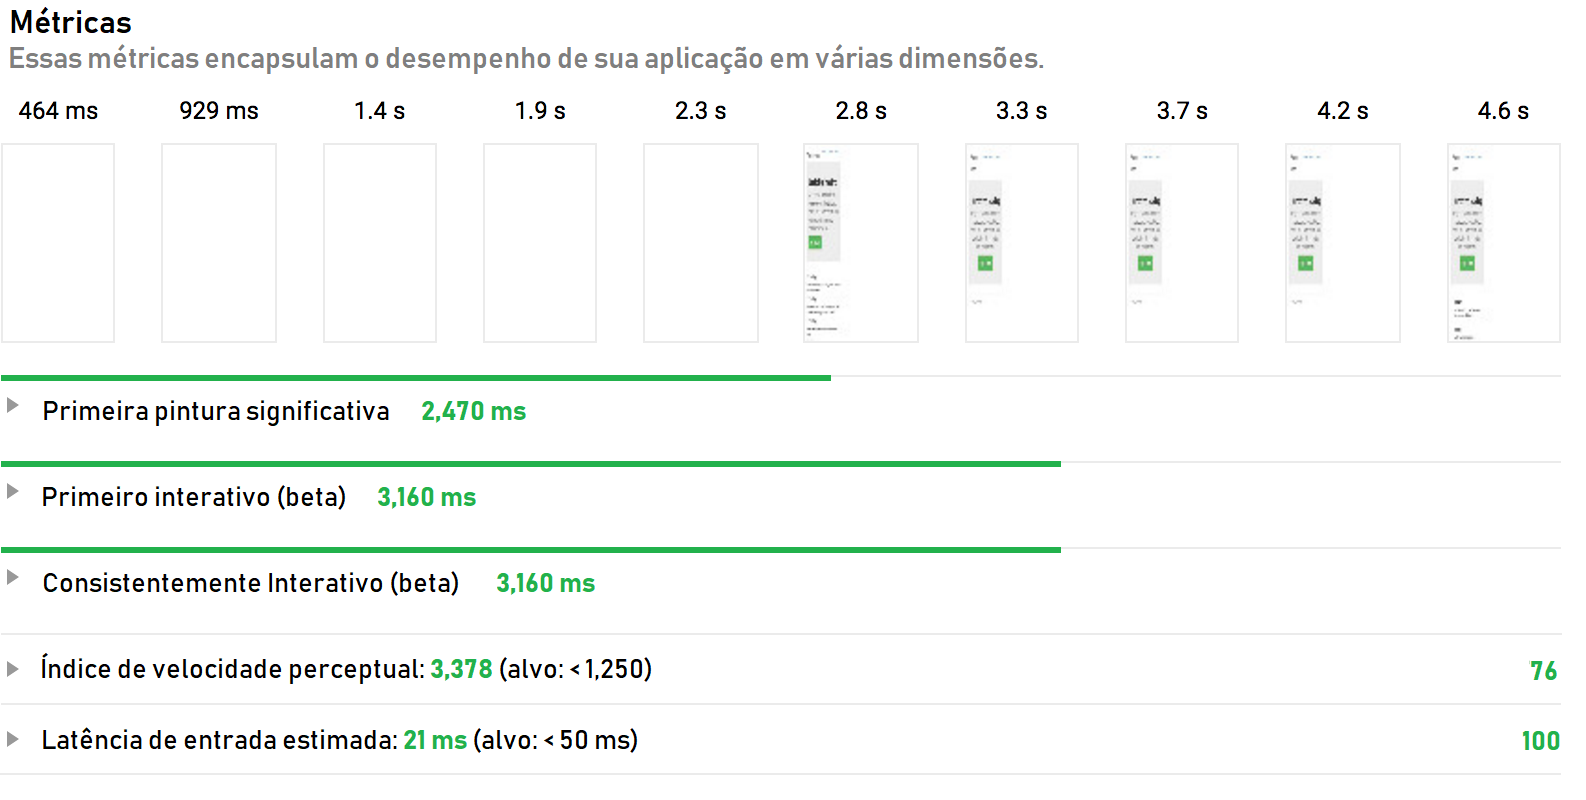
\includegraphics[width=0.75\textwidth]{figuras/critical_css_before}
\begin{flushleft}
\flushleft{Fonte: Gerado no \textit{Lighthouse}, por Anthony Gore.}
\end{flushleft}
\label{fig:withoutcritical}
}
\end{figure}

O desempenho da renderização, é medido através da ferramenta \textit{Lighthouse}~\footnote{Disponível em: https://goo.gl/H8EpEJ. Data de Acesso: 18 de Abril de 2018.}, uma extensão para navegador, automatizada e de código fonte aberto. A \textit{Lighthouse} é desenvolvida e mantida pela mesma equipe responsável pelo Google Chrome, e a mesma é utilizada para auditar a qualidade de renderização das páginas \textit{Web}. Através da utilização desta ferramenta, foi gerado um relatório, apresentado na Figura~\ref{fig:withoutcritical}, que lista métricas utilizadas para medir o desempenho da renderização da página \textit{Web}, tais como: Primeira pintura significativa~\footnote{Tempo necessário para que o conteúdo principal de uma página seja visível.}; Eventos de interação~\footnote{Tempo em que a página torna-se interativa.}; Índice de velocidade perceptual~\footnote{Velocidade com que o conteúdo de uma página é visivelmente preenchida.} e Latência de entrada estimada~\footnote{Tempo, em milissegundos, que a aplicação necessita para responder a entrada no usuário.}. Todavia, apenas o comportamento da primeira pintura significativa é avaliada, devido ao impacto causado pela técnica testada sobre a métrica. Em outras palavras, devido ao tempo que leva até que o usuário possa perceber conteúdo na página. Na Figura~\ref{fig:withcritical}, pode-se perceber a melhoria do desempenho após o isolamento do CSS crítico do restante da folha de estilos em cascata.

\begin{figure}[th]
\centering{
\caption{Desempenho depois do \textit{Critical} CSS.}
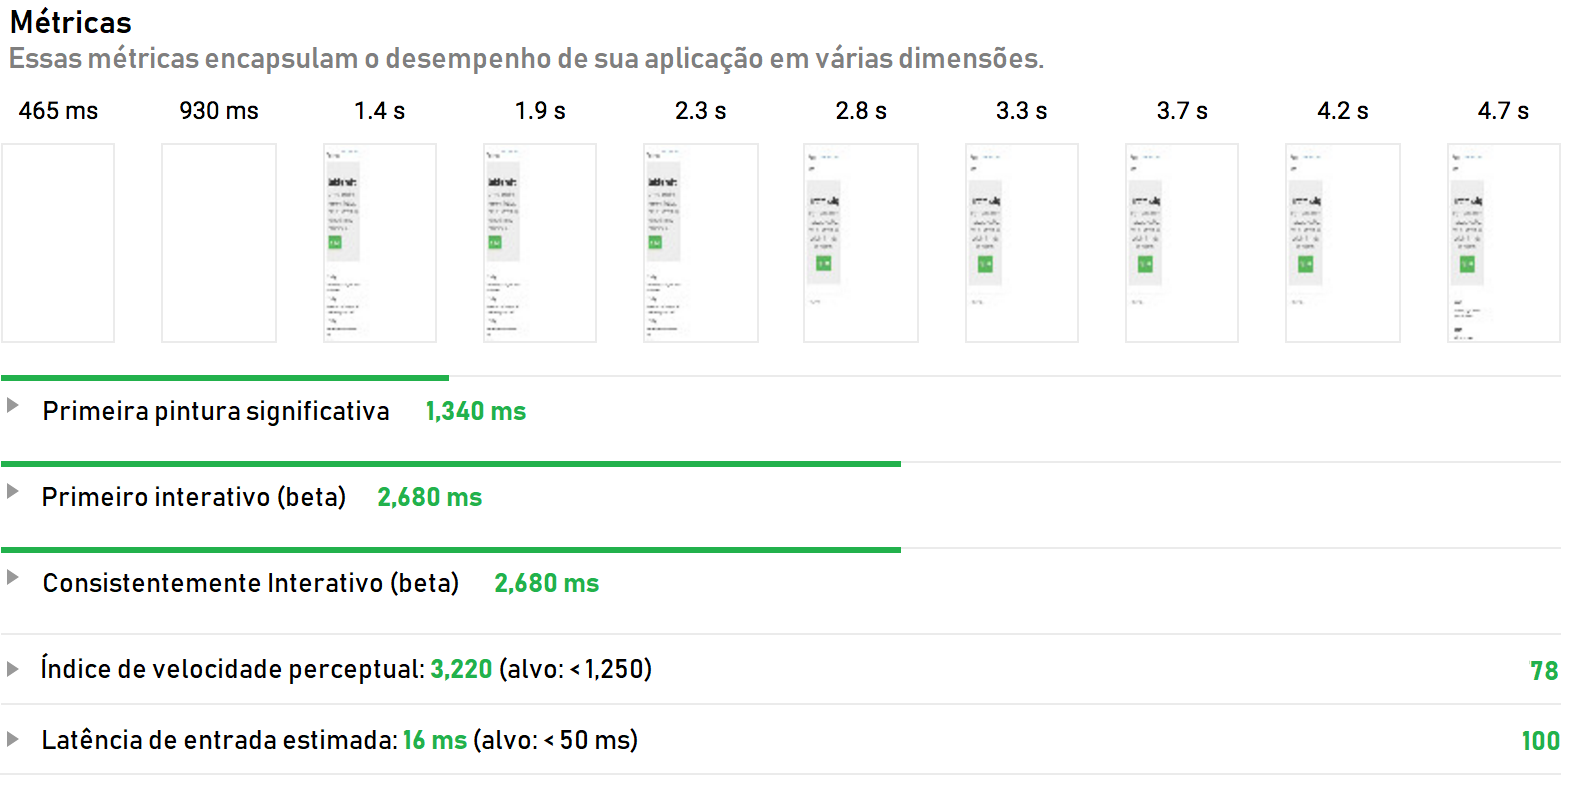
\includegraphics[width=0.75\textwidth]{figuras/critical_css_after}
\begin{flushleft}
\flushleft{Fonte: Gerado no \textit{Lighthouse}, por Anthony Gore.}
\end{flushleft}
\label{fig:withcritical}
}
\end{figure}

Logo após a implementação da técnica de \textit{Critical} CSS, é possível observar uma diminuição significativa no tempo necessário para a primeira pintura de página. Esta redução, foi de, aproximadamente, 54\% em relação ao mesmo resultado antes da aplicação da técnica. É perceptível tal otimização, pois o tempo necessários para a apresentação primeiro efeito visual foi reduzido de 2470ms para 1340ms. Esta melhoria, proposta por Anthony Gore, reduziu, também, o tempo necessário para a liberação dos eventos de interação na página, que podem ser manipulados pelo usuário ou por animações. Além destes eventos de interatividade, as métricas de Latência de entrada estimada e Índice de velocidade perceptual, sofreram variações. Entretanto, não há melhora significativa, para estas últimas métricas. Porém a aplicação da técnica não compromete o desempenho das outras métricas auditadas.

Os resultados foram obtidos a partir de um documento HTML com a adição de uma biblioteca CSS (\textit{Bootstrap}), aproximadamente 217 \textit{kilobytes} (que é um tamanho considerável para uma página simples de testes). A escolha da biblioteca é arbitrária e pode ser substituída por qualquer código CSS. Outras métricas podem ser obtidas a partir da extensão \textit{Lighthouse}, porém, não agregam valor à proposta inicial deste trabalho. Devido a este fato, novos resultados não foram adicionados, restando apenas cinco otimizações que culminaram em sucesso após a aplicação da técnica.

O Capítulo~\ref{Proposta}, também apresenta outra otimização importante, que é a redução do \textit{payload}. Essa estratégia utiliza um conjunto de técnicas voltadas à otimização do desempenho de renderização da página, que incluem: Redução do número de requisições realizadas; Redução da quantidade de dados enviados nas requisições; Aglomeração de arquivos do mesmo tipo; Compressão GZIP pelo servidor; Compressão do código gerado.

O ambiente de testes é fornecido pela Lux Teams~\footnote{Disponível em: https://app.teamslux.com/. Data de Acesso: 12 de Abril de 2018.}, um sistema integrado de gerência de reuniões, acompanhamento de projetos e tarefas. Bem como, a utilização do \textit{Firefox Developer Edition}~\footnote{Disponível em: https://www.mozilla.org/pt-BR/firefox/channel/desktop/. Data de Acesso: 18 de Abril de 2018.}, um navegador criado para atender as necessidades dos desenvolvedores \textit{Web} em seus testes. Os experimentos propostos, utilizam duas versões do sistema, que são: Versão 1.0, desenvolvida sem \textit{code-pattern} e não otimizada; Versão atual (2.1), apesar de não concluída, esta versão, está em fase avançada e os resultados de performance não são interferidos, visto que as métricas utilizadas estão estáveis. Além deste fato, a nova versão utilizou (desde o início do desenvolvimento), \textit{code-pattern} e otimizações. A seguir, é detalhada a redução do \textit{payload} nesta comparação.

\begin{figure}[th]
\centering{
\caption{\textit{Payload} antes da otimização.}
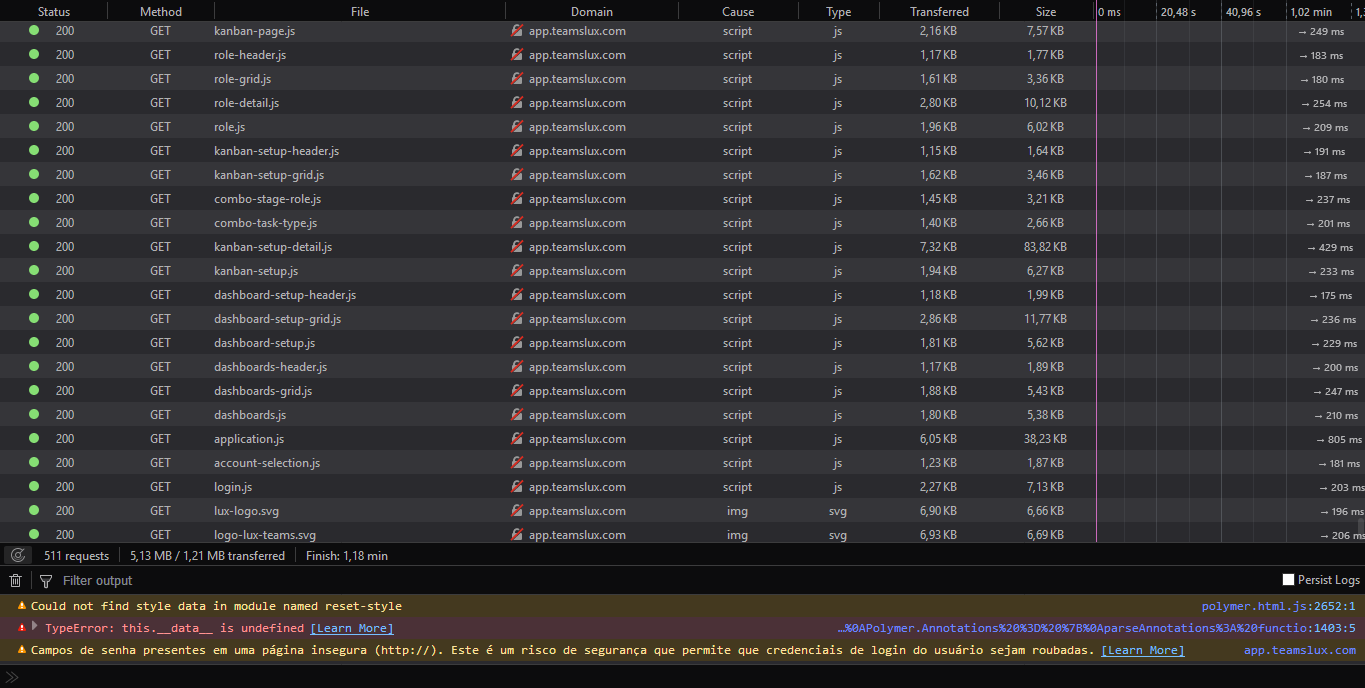
\includegraphics[width=1\textwidth]{figuras/oldlux.png}
\begin{flushleft}
\flushleft{Fonte: Disponibilizado pelo Autor.}
\end{flushleft}
\label{fig:oldlux}
}
\end{figure}

Nas Figuras~\ref{fig:oldlux}~e~\ref{fig:newlux}, podem ser observadas, o número de requisições realizadas a partir da entrada com credenciais no sistema (\textit{Login}) até o carregamento completo da tela principal. Além do \textit{payload} e o tempo de transferência necessário para o recebimento de todas as requisições. Os experimentos foram realizados múltiplas vezes para obter-se um resultado justo, com base na média. Além disso, a leitura de desempenho foi medida em horários de menor pico, de forma que, a interferência de rede seja mínima para o resultado final do teste realizado.

O \textit{payload} antes da otimização, na Figura~\ref{fig:oldlux}, possuía 5,13 \textit{megabytes} correspondentes com as 511 requisições disparadas. O tempo de resposta de todas as requisições durou aproximadamente 71 segundos (1,18 minuto), o que é lento. Após implementar as modificações propostas para a redução do \textit{payload}, pode-se observar na Figura~\ref{fig:newlux}~o resultado desta otimização.

\begin{figure}[th]
\centering{
\caption{\textit{Payload} depois da otimização.}
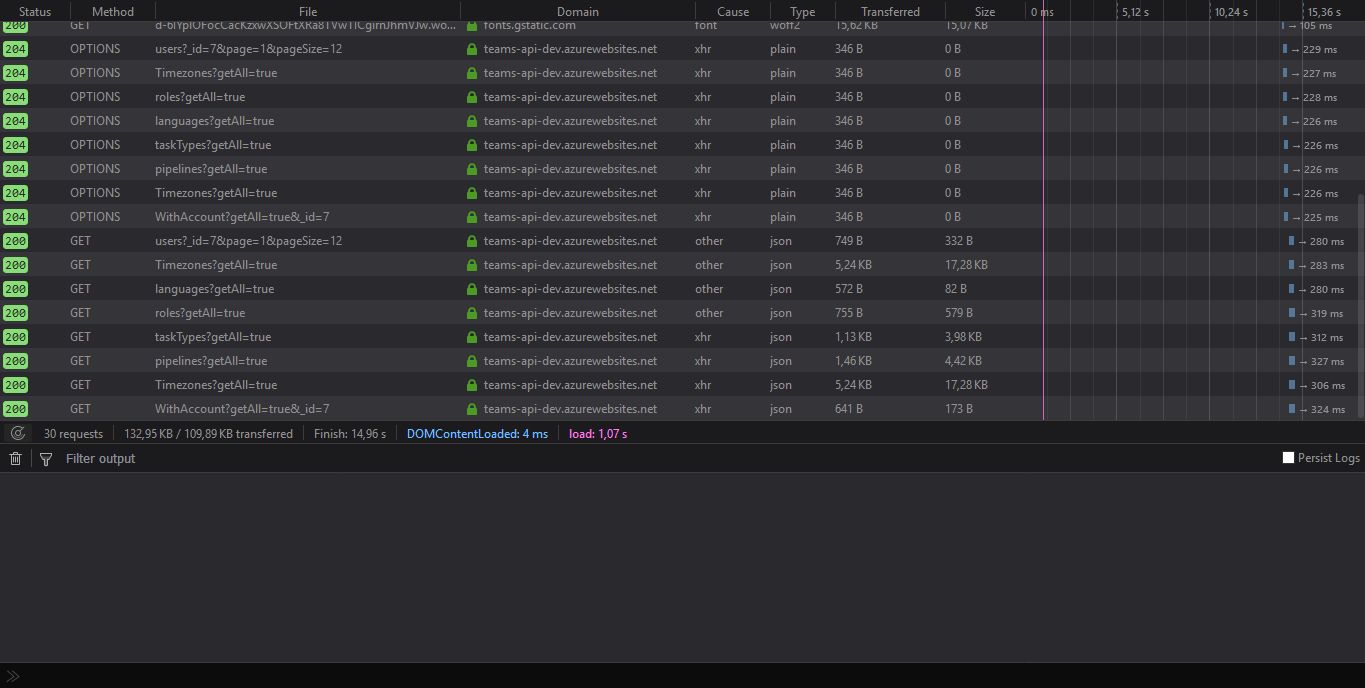
\includegraphics[width=1\textwidth]{figuras/newlux.png}
\begin{flushleft}
\flushleft{Fonte: Disponibilizado pelo Autor.}
\end{flushleft}
\label{fig:newlux}
}
\end{figure}

Ao final de todas as implementações, observa-se uma redução significativa em todas as métricas avaliadas na Figura~\ref{fig:newlux}. Antes da otimização, haviam 511 requisições. Já após a otimização, esse número foi reduzido para 30 requisições, 5.87\% do número total de requisições. Além da diminuição da duração total da requisição para apenas 15 segundos, 21.1\% do tempo total de aproximadamente 71 segundos. Esta redução pode ser explicada pela necessidade de consumir o recurso da API REST apenas quando solicitado. Em outras palavras, foi observado que, várias requisições poderiam ser solicitadas por demanda, não havendo necessidade em requisitar todo o conteúdo após a entrada no sistema, o que impactava, inclusive, o carregamento da página inicial. Além desta métrica, o tamanho de dados a serem transferidos, bem como o tempo necessário para todas as requisições serem finalizadas foram reduzidos. Este comportamento deve-se principalmente à redução do número total de requisições. É pertinente observar que ao utilizar-se da Internet para trafegar os dados, a Aplicação \textit{Web} está sucessível a erros e complicações de rede ligados diretamente ao modo que os protocolos que compõem a Internet operam. Isto é, lentidão na entrega causadas por congestionamentos de rede, perca de pacotes, latência na entrega devido a múltiplos saltos, tamanho das requisições e respostas. Todas essas problemáticas são inevitáveis e estão presentes em qualquer rede de computadores convencional ao modelo TCP/IP que é difundido por toda Internet. Entretanto, otimizações podem ser aplicadas, assim como neste trabalho, a fim de diminuir o impacto de um eventual problema de rede. Sendo assim, o usuário final observará um menor atraso na exibição de dados, o que contribui diretamente para melhorar a usabilidade da aplicação em questão.